\documentclass[a4paper,leqno,12pt]{amsart}
%
\usepackage{amsmath,amsthm}
\usepackage{graphicx}
\usepackage[margin=0.7in]{geometry}

\usepackage{enumitem}

\usepackage{comment}
\usepackage{multirow}
\usepackage{tikz}
\usepackage{wrapfig}
\usepackage[autostyle=true]{csquotes}

\usepackage{pgfplots}
\usepackage{pgf-pie} % simple and featureful for pie charts
\pgfplotsset{compat=1.18}
\usepackage{filecontents} % only needed for the external-data example


\usepackage{fancyhdr}
\pagestyle{fancy}
\fancyhf{} % clear all header/footer fields
\fancyfoot[C]{\bf ************************************} % 

\newlist{Case}{enumerate}{1}
\setlist[Case]{label=\bf{Case ~\arabic*:}}
%
\begin{document}
\hspace*{1.9cm}% <-- adjust this value to push everything right
\begin{tabular}{@{}p{0.7\textwidth}p{0.3\textwidth}@{}}
 {\raggedright
   \begin{center} 
   \textbf{AZIM PREMJI UNIVERSITY, BHOPAL}\\
   First Semester 2026--2027 \\
   Tutorial Sheet--8
   \end{center}
  } %&
  %{\raggedleft
   %
\includegraphics[width=3cm]{Azim_Premji_University_logo.png} % replace logo.png with your file name
  %}
\end{tabular}


\noindent Course No. MTH-113 \hfill  Course title: Introduction to Quantitative Thinking
\vspace{.3cm}
\hrule 
\vspace{.3cm}


\begin{enumerate}
\setlength\itemsep{1em}
\item In a Mathematics test, the following marks were obtained by 40 students. Arrange
these marks in a table using tally marks.

\begin{center}
  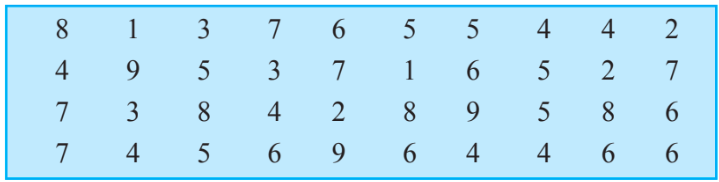
\includegraphics[width=0.6\textwidth]{QS-TS8-Q1.png}
\end{center}

\begin{enumerate}
 \item Find how many students obtained marks equal to or more than 7.
 \item How many students obtained marks below 4?
\end{enumerate}

\item Following is the choice of sweets of 30 students of Class VI.
\vspace{1.5mm}\\
Ladoo, Barfi, Ladoo, Jalebi, Ladoo, Rasgulla, Jalebi, Ladoo, Barfi, Rasgulla, Ladoo,
Jalebi, Jalebi, Rasgulla, Ladoo, Rasgulla, Jalebi, Ladoo, Rasgulla, Ladoo, Ladoo,
Barfi, Rasgulla, Rasgulla, Jalebi, Rasgulla, Ladoo, Rasgulla, Jalebi, Ladoo. 
\vspace{1.5mm}
\begin{enumerate}
 \item Arrange the names of sweets in a table using tally marks.
 \vspace{1.5mm}
 \item Which sweet is preferred by most of the students?
\end{enumerate}

\item Catherine threw a dice 40 times and noted the number appearing each time as
shown below:
\begin{center}
 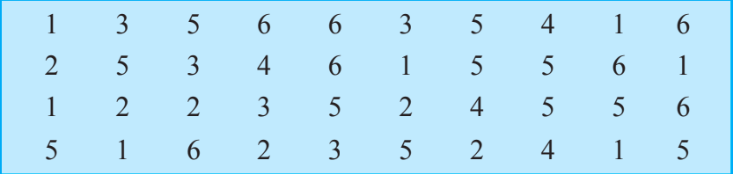
\includegraphics[width=0.6\textwidth]{QS-TS8-Q3.png}
\end{center}
\vspace{0.1mm}
Make a table and enter the data using tally marks.
\vspace{1mm}
\begin{enumerate}
 \item Find the number that appeared the minimum number of times 
 \vspace{1mm}
 \item Find the number that appeared the maximum number of times
 \vspace{1mm}
 \item Find those numbers that appear an equal number of times.
\end{enumerate}

\item The number of girl students in each class of a co-educational middle school is depicted
by the pictograph:
\begin{center}
 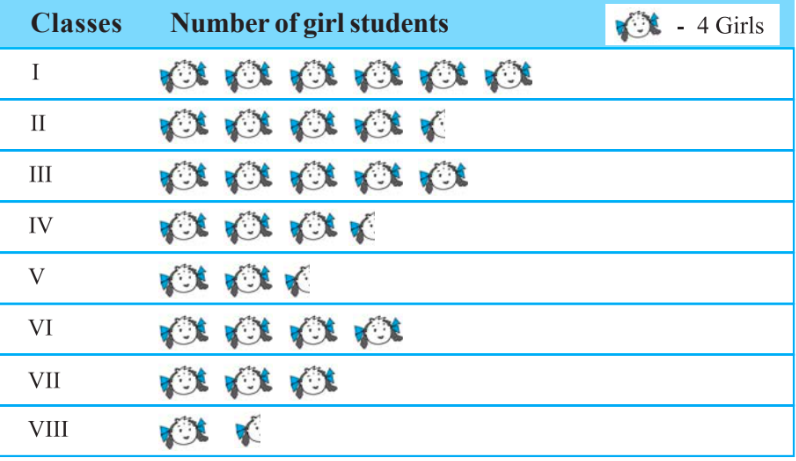
\includegraphics[width = 0.6\textwidth]{QS-TS8-Q4.png}
\end{center}
\vspace{0.1mm}
Observe this pictograph and answer the following questions:
\begin{enumerate}
 \item Which class has the minimum number of girl students?
 \item Is the number of girls in Class VI less than the number of girls in Class V?
 \item How many girls are there in Class VII?
\end{enumerate}

\item A survey of 120 school students was done to find which activity they prefer
to do in their free time.

\begin{center}
\begin{tabular}{|c|c|c|}
  \hline
  \textbf{Preferred activity} & \textbf{Number of students} \\
  \hline
  Playing & 45 \\
  Reading story books & 30 \\
  Watching TV & 20 \\
  Listening to music & 10 \\
  Painting & 15 \\
  \hline
\end{tabular}
\end{center}
\vspace{1mm}
Draw a bar graph to illustrate the above data taking scale of 1 unit
length = 5 students.
Which activity is preferred by most of the students other than playing?

\item The number of Mathematics books sold by a shopkeeper on six consecutive
days is shown below:
\begin{center}
\begin{tabular}{|c|c|c|c|c|c|c|}
 \hline
 \textbf{Days} & \text{Sunday} & \text{Monday} & \text{Tuesday} & \text{Wednesday} & \text{Thursday} & \text{Friday}\\
 \hline
 \textbf{Number of Books Sold} & 65 & 40 & 30 & 50 & 20 & 70 \\
 \hline
\end{tabular}
\end{center}
\vspace{1mm}
Draw a bar graph to represent the above information choosing the scale of
your choice.


\item Following table shows the number of bicycles manufactured in a factory during
the years 1998 to 2002. Illustrate this data using a bar graph. Choose a scale of
your choice.
\vspace{1mm}
\begin{center}
\begin{tabular}{|c|c|}
 \hline
 \textbf{Years} & \textbf{Number of bicycles manufactured} \\
 \hline
 1998 & 800 \\
 1999 & 600 \\
 2000 & 900 \\
 2001 & 1100 \\
 2002 & 1200 \\
 \hline
\end{tabular}
\end{center}
\vspace{2mm}
\begin{enumerate}
 \item In which year were the maximum number of bicycles manufactured?
 \vspace{1mm}
 \item In which year were the minimum number of bicycles manufactured?
\end{enumerate}

\item Number of persons in various age groups in a town is given in the following table.
\begin{center}
\begin{tabular}{|c|c|c|c|c|c|c|}
 \hline
 \textbf{Age group} & \text{1-14} & \text{15-29} & \text{30-44} & \text{45-59} & \text{60-74} & \text{75 and above}\\
 \hline
 \textbf{Number of } & \text{2 lakhs} & \text{1 lakhs} &  \text{1 lakhs} & \text{1 lakhs} & 80 & 40 \\
 \textbf{Persons} & & \text{60 thousands} & \text{20 thousands} & {20 thousands} & & \text{thousands} \\
 \hline
\end{tabular}
\end{center}
\vspace{2mm}
Draw a bar graph to represent the above information and answer the following questions.
(take 1 unit length = 20 thousands)
\vspace{2mm}
\begin{enumerate}
 \item Which two age groups have same population?
 \vspace{1mm}
 \item All persons in the age group of 60 and above are called senior citizens. How many
senior citizens are there in the town?
\end{enumerate}


\item For which of these would you use a histogram to show the data?
\begin{enumerate}
 \item The number of letters for different areas in a postman’s bag.
 \item The height of competitors in an athletics meet.
 \item The number of cassettes produced by 5 companies.
 \item The number of passengers boarding trains from 7:00 a.m. to 7:00 p.m. at a station.
\end{enumerate}
\vspace{1mm}
Give reasons for each.

\item The weekly wages (in Rs) of 30 workers in a factory are.\\
830, 835, 890, 810, 835, 836, 869, 845, 898, 890, 820, 860, 832, 833, 855, 845,
804, 808, 812, 840, 885, 835, 835, 836, 878, 840, 868, 890, 806, 840.\\
Draw a histogram for the frequency table made for the above data, and
answer the following questions.
\begin{enumerate}
 \item Which group has the maximum number of workers?
 \item How many workers earn Rs 850 and more?
 \item How many workers earn less than Rs 850?
\end{enumerate}

\item The number of hours for which students of a particular class watched television during
holidays is shown through the given graph.\\
\vspace{1mm}
Answer the following.
\begin{enumerate}
 \item For how many hours did the maximum number of students watch TV?
 \item How many students watched TV for less than 4 hours?
 \item How many students spent more than 5 hours in watching TV?
\end{enumerate}

\vspace{3mm}

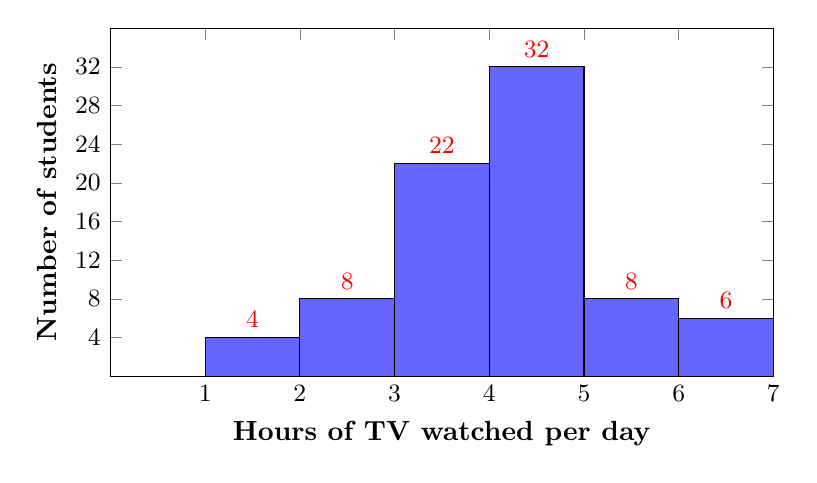
\begin{tikzpicture}
  \begin{axis}[
    width=10cm,
    height=6cm,
    ymin=0,
    ymax=36,
    xmax=7,
    ylabel={\textbf{Number of students}},
    xlabel={\textbf{Hours of TV watched per day}},
    xtick={1,2,3,4,5,6,7},
    ytick={4,8,12,16,20,24,28,32},
    yticklabel style = {font=\small},
    xticklabel style={font=\small},
    ymajorgrids=false,
    %grid style={gray!20},
    enlarge x limits=false,
  ]
    % ybar interval: each coordinate (x_i,y_i) sets the height for the interval [x_i,x_{i+1}]
    \addplot+[ybar interval, draw=black, fill=blue!60, mark=none] coordinates {
      (0,0)	
      (1,4) % height 4 on interval [1,2]
      (2,8) % height 8 on interval [2,3]
      (3,22) % height 0 on interval [3,?]
      (4,32)
      (5,8)
      (6,6)
      (7,0)
    };
    \addplot+[only marks, mark=none, nodes near coords, point meta=explicit,
              nodes near coords style={font=\small, yshift=0pt},
              forget plot] coordinates {
      (1.5,4)  [4]
      (2.5,8)  [8]
      (3.5,22) [22]
      (4.5,32) [32]
      (5.5,8)  [8]
      (6.5,6)  [6]
    };
  \end{axis}
\end{tikzpicture}

\item A survey was made to find the type of music
that a certain group of young people liked in
a city. Following pie chart shows the findings
of this survey.

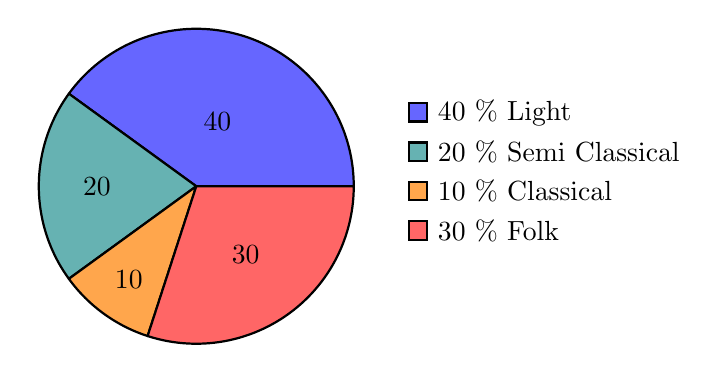
\begin{tikzpicture}
  \pie[
    /tikz/every pin/.style={align=center,mark=none,font=\small},
    text=legend,            % show labels in a legend style
    radius=2,               % radius of the pie
    color={blue!60, teal!60, orange!70, red!60}, % slice colors
    sum=auto,               % compute percentages automatically
    explode={0.0,0.0,0.0,0.0} % slightly separate the 2nd slice
  ]{
    40/40 \% Light,   % value / label
    20/20 \% Semi Classical,
    10/10 \% Classical,
    30/30 \% Folk
  }
\end{tikzpicture}

From this pie chart answer the following:
\begin{enumerate}
 \item If 20 people liked classical music, how
many young people were surveyed?
 \item Which type of music is liked by the
maximum number of people?
 \item If a cassette company were to make
1000 CD’s, how many of each type
would they make?
\end{enumerate}


\item Draw a pie chart showing the following information. The table shows the colours
preferred by a group of people.
\begin{center}
\begin{tabular}{|c|c|}
 \hline
 \textbf{Colours} & \textbf{Number of People} \\
 \hline
 \text{Blue} & 18 \\
 \text{Green} &  9 \\
 \text{Red} & 6 \\
 \text{Yellow} & 3 \\
 \hline
 \textbf{Total} & 36 \\
 \hline
\end{tabular}
\end{center}

\item List the outcomes you can see in these experiments.\\
(a) Spinning a wheel $\hfill$ (b) Tossing two coins together
\[
 \hspace*{-2cm}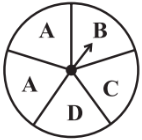
\includegraphics[width=0.2\textwidth]{QS-TS8-Q14.png}
\]

\item When a die is thrown, list the outcomes of an event of getting\\
(a) a prime number \hspace*{3cm} (b) not a prime number\\
(c) a number greater than 5 \hspace*{1.5cm} (d) a number not greater than 5.

\item Find the.
\begin{enumerate}
 \item Probability of the pointer stopping on D in (Question 14-(a))?
 \item Probability of getting an ace from a well shuffled deck of 52 playing cards?
 \item Probability of getting a red apple. (See figure below)
\end{enumerate}
\vspace{3mm}
\[
 \hspace*{-2cm}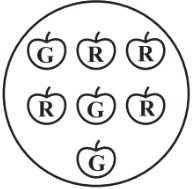
\includegraphics[width=0.2\textwidth]{QS-TS8-Q15.png}
\]


\end{enumerate}


%\vspace*{0.2cm}
%\begin{center}
%{\bf ************************************}
%\end{center}

\end{document}